\chapter{Developed Models}
\label{chap:Models}

This chapter aims to explore two key elements in time series analysis: data preparation and model architectures. Effective manipulation and organization of information is a key prerequisite to facilitate learning from a forecasting model due to the high complexity of temporal data. The first section of this chapter will focus on the methodology and techniques used to prepare temporal data, outlining selected practical approaches to address specific challenges noted in the chosen data.

The following section will shift the focus to model architectures. Several architectural paradigms will be examined, with particular emphasis on advanced solutions that have demonstrated significant impact in the time series prediction task, some already anticipated in Section \ref{cap1:sota}.

\section{Data Preparation}
\label{sec:DataPreparation}

The principal function of data preparation is to locate relevant characteristics in datasets and then modify the data in order to maximize model performance. This crucial procedure comes before model training, greatly enhancing the prediction power of the models.

To extract pertinent information from raw data, which is frequently heterogeneous and unstructured, considerable selection is required. Data cleansing, controlling outliers, addressing missing values, and guaranteeing data consistency are all part of the first step of data preparation. By interacting, these measurements help to create a more refined dataset, which serves as the foundation for further analytical procedures.

\subsection{Feature engineering and selection}
Feature selection and design in a machine learning model involves choosing the most important features for the model and creating ad hoc features to aid learning. 
\textbf{Feature selection} is the process of selecting a subset of relevant features for use in building the model.
Feature selection techniques are used for several reasons, including simplifying models to make them more easily interpretable, reducing training times, and avoiding the curse of dimensionality.
In our case, feature selection is utilized to eliminate redundant exogenous variables based on their correlation.
For example, in CityPulse, feelslike and occupied variables are removed, while temp and occupancy are kept. In Seoul and Madrid, rain is kept and prec is removed.
On the other hand, \textbf{feature engineering} involves extracting features from raw data to support training.
In this case, feature engineering is utilized to extract \textbf{date-based features}, such as the day of the week, month of the year, and time of day. These features can be valuable for forecasting. As we have observed, many pollutants tend to have lower values during weekends. Therefore, incorporating the day of the week as a feature can improve the accuracy of the forecasting model.


After the extraction of the date-based features, these are converted to multiple one-hot encoded variables. \textbf{One-hot encoding} is a technique that encodes using a dummy encoding scheme. This means creating a binary column for each category and the result is a sparse matrix of 0s and 1s, based on the original value of the column (example in Figure \ref{fig:one-hot}).
\begin{figure}
    \centering
    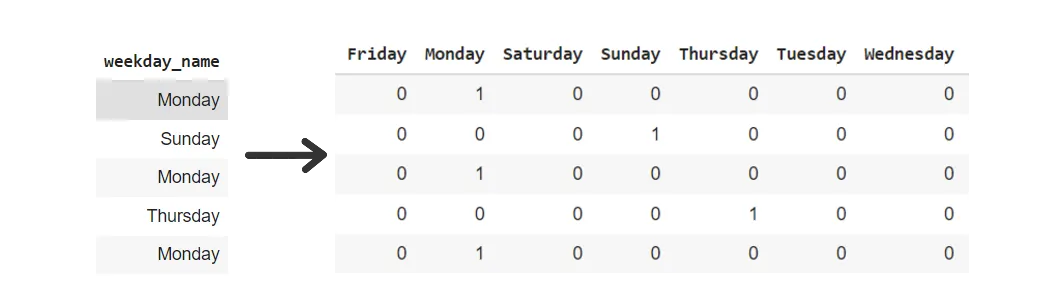
\includegraphics[width=0.75\linewidth]{images/onehotencoding.png}
    \caption{One-hot encoding sample illustration \cite{onehotencoding}}
    \label{fig:one-hot}
\end{figure}

\subsection{Data scaling}

Data scaling is the process of \textbf{adjusting the range of values} in a dataset to ensure that all variables contribute equally to the analysis. It prevents certain features from dominating others due to differences in their scales. Common scaling techniques include Min-Max scaling, where values are normalized to a specific range, and Z-score normalization (formula found in Figure \ref{eq:standardization}), which standardizes data to have a mean of 0 and a standard deviation of 1. The latter is used in this work.

\begin{figure}
\[ z_{ij} = \frac{{x_{ij} - \bar{x}_j}}{{\sigma_j}} \]
\caption{Z-score normalization formula}
\label{eq:standardization}
\end{figure}
\text{Where:}
\begin{itemize}[noitemsep, leftmargin=*]
  \item[] $z_{ij}$ \text{ is the normalized value in the } i\text{-th row and } j\text{-th column.}
  \item[] $x_{ij}$ \text{ is the original value in the } i\text{-th row and } j\text{-th column.} 
  \item[] $\bar{x}_j$ \text{ is the mean of the } j\text{-th column.} 
  \item[] $\sigma_j$ \text{ is the standard deviation of the } j\text{-th column.}
\end{itemize}


\paragraph{}Z-score normalization brings several benefits to the training of deep learning models. First and foremost, it promotes convergence by accelerating the optimization process. Normalizing features to a common scale enables the model to navigate the parameter space more efficiently, facilitating \textbf{faster convergence} during gradient-based optimization.

Additionally, as said, z-score normalization aids in stabilizing the training process by \textbf{preventing certain features }from\textbf{ dominating others}. In datasets with disparate feature scales, the influence of larger magnitude features can overshadow smaller ones. This dominance can lead the model to prioritize certain features, neglecting others and resulting in suboptimal generalization. Z-score normalization mitigates this issue by equalizing the impact of all features.

\subsection{Data augmentation}
\label{subsec:data-augmentation}

Data augmentation is a technique commonly used in deep learning to artificially increase the diversity of a training dataset. The idea is to apply various transformations to the existing training data, creating new, slightly modified versions of the original samples. This process helps the model generalize better to unseen data and improves its robustness.
In the context of this research project, the application of a data augmentation technique known as jittering was examined across three datasets. Jittering involves the introduction of random noise into the time series. Specifically, to each observation, a random value drawn from a Gaussian distribution with a mean of 0 and a standard deviation ranging from 0 to 0.2 was added. Importantly, this standard deviation varied at each epoch during the training process.

\begin{figure}
\[X_{\text{jittered}, i} = X_i + \epsilon_i\]
\label{eq:jittering}
\end{figure}
Where: 
\begin{itemize}[noitemsep, leftmargin=*]
    \item[] $X_{\text{jittered}, i}$ represents the \(i\)-th data point in the jittered time series
    \item[] \(X_i\) is the \(i\)-th data point in the original time series
    \item[] \(\epsilon_i\) is the random noise sampled from a Gaussian distribution
\end{itemize}

\begin{figure}
    \centering
    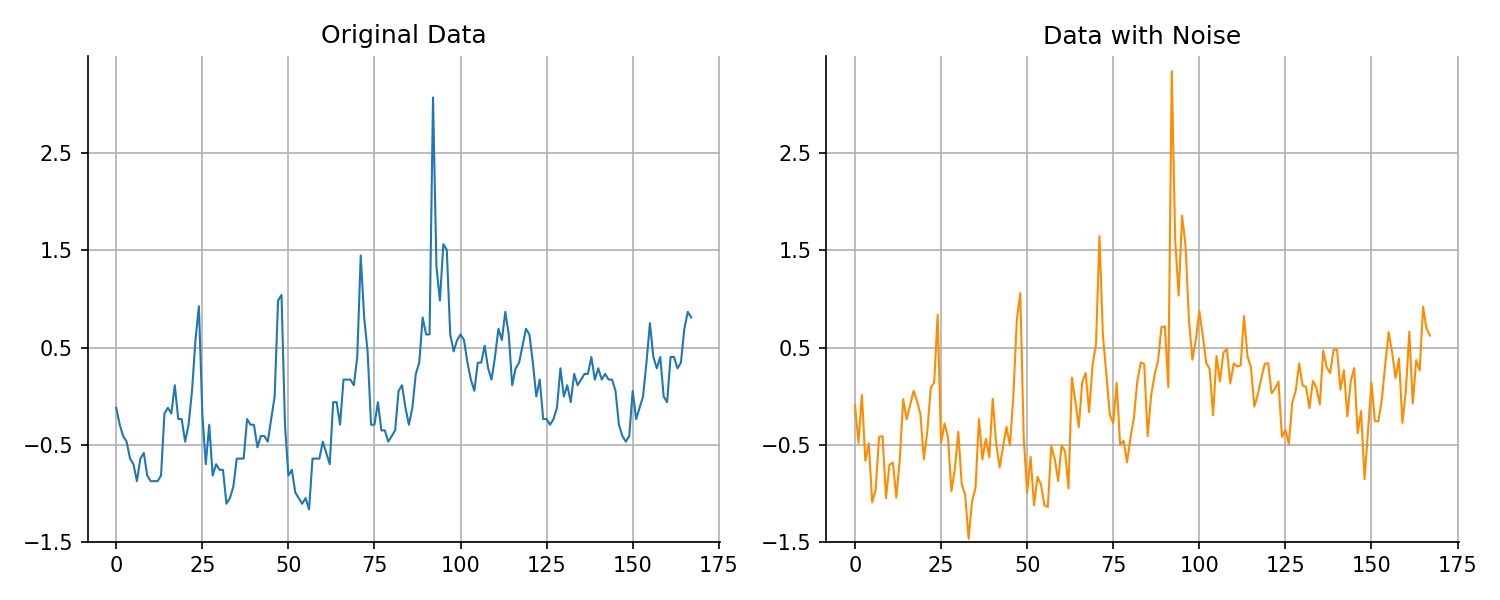
\includegraphics[width=0.75\linewidth]{images/jittering.png}
    \caption{Example of jittering in time series data, with random noise from Gaussian distribution $\mu = 0$ and $\sigma = 0.2$}
    \label{fig:jittering}
\end{figure}


\subsection{Data splitting}

The research question of this work involves a multivariate multi-step forecasting task. In practical terms, this means using past observations at time $t_{past}$ to predict $t_{future}$ future observations. Typically, the time window used for $t_{past}$ is greater than or equal to the time window used for $t_{future}$.
In our case, we employ a technique that transforms the dataset from unsupervised to supervised. A dataset for supervised learning contains one or more target variables, each assigned to a set of independent variables.
In all experiments, we used 168 past observations (24 observations per day for 7 days) to forecast 24 future observations (1 day).

Regarding the data used for model training, it was divided into 3 temporally ordered splits:
\begin{itemize}
    \item Training data (first 80\% of the data)
    \item Validation data (10\% of the data)
    \item Test data (10\% of the data)
\end{itemize}

For time series forecasting tasks, it is crucial that the data sampling for each set is not random. Instead, the data should be extracted in chronological order. This is to prevent the model from being exposed to data that will later need to be forecasted in the validation and test sets, ensuring results that are faithful to real-world scenarios.

The introduction of noise in the data takes place online during the training phase, and it is added to each batch individually.

\subsection{Experiments}
\label{subsec:experiments}
While the following section will present the tested models, this section will briefly discuss the examined time horizons. The objective is to assess the effectiveness of the models not only across various cities, each characterized by distinct pollutant distribution patterns, but also in relation to the volume of historical data available. Therefore, the aim is to determine whether and to what extent the possession of more or less historical data influences the accuracy of predictions.

Additionally, the study aimed to assess the effectiveness of the models using both original and noise-augmented data. A summary table of the experiments conducted is presented in Table \ref{tab:dataset_testing}.


\begin{table}[h]
  \centering
  \begin{tabular}{|c|c|c|c|}
    \hline
    \textbf{Dataset} & \textbf{Time Horizon} & \textbf{Original Data} & \textbf{Data with noise} \\ 
    \hline
    Seoul & 1 year & \checkmark &  \\
     & 3 years & \checkmark & \checkmark \\    \hline
    Madrid & 1 year & \checkmark &  \\
     & 3 years & \checkmark & \checkmark \\    \hline
    Citypulse & 3 months & \checkmark & \checkmark \\
    \hline
  \end{tabular}
  \caption{Temporal and Data Variation in Model Testing}
  \label{tab:dataset_testing}
\end{table}

\section{Model architectures}

Deep learning models are known for their complex architectures, which consist of multiple layers and numerous parameters. The interaction of these components can introduce a high degree of variability in the performance of different models, even when they are trained on the same dataset. Therefore, it is essential to use rigorous testing procedures to evaluate the effectiveness of various architectures. Evaluations are based on objective metrics such as error, as well as considerations of generalization and computational efficiency.
Various architectures, from basic to modern, have been tested for their effectiveness, efficiency, and generalization capability.

\subsection{ARIMA}
\label{subsec:baseline}

To provide an overall comparison between the models proposed, an ARIMA model has been developed, which, taking as input one pollutant at once, together with other variables, including the time-based features, predicts the variable for multiple steps over time. 
The Autoregressive Integrated Moving Average (ARIMA) model is a traditional time series forecasting technique developed by Box and Jenkins \cite{box1970time}. It combines autoregression (AR), differencing (I), and moving averages (MA). The general form is ARIMA(p, d, q), where p is the autoregressive order, d is the differencing order, and q is the moving average order. The model equation is the following:
\begin{align*}
(1 - \phi_1 L - \dots - \phi_p L^p)(1 - dL)^d Y_t = c + \theta_1 \varepsilon_{t-1} + \dots + \theta_q \varepsilon_{t-q} + \beta_1 X_{1,t} + \dots + \beta_k X_{k,t}
\end{align*}
Where: 
\begin{itemize}[leftmargin=*, noitemsep]
    \item[] $Y_t$ is the time series value at time $t$
    \item[] $L$ is the lag operator, such that $L^k Y_{t-k} = Y_{t-k}$ 
    \item[] $\phi_1, \dots ,  \phi_p$ are the autoregressive (AR) parameters
    \item[] $d$ is the differencing order (integrated part)
    \item[] $\theta_1, \dots , \theta_q$ is the  moving average (MA) parameters
    \item[] $c$ is the optional constant term (intercept)
    \item[] $\varepsilon_t$ is the white noise error term at time $t$
    \item[] $X_{1,t}$, \dots, $X_{k,t}$ are  the external regressors or exogenous variables at time $t$. 
    \item[] $\beta_1$, \dots, $\beta_k$ are the coefficients associated with the external regressors.
\end{itemize}



ARIMA is a commonly used method for time series forecasting because of its adaptability and interpretability. The model's parameters (p, d, q) are determined through an automated process called auto-ARIMA, which uses algorithmic methods to select the optimal values of p, d, and q based on the minimization of a metric, typically the Akaike Information Criterion (AIC). This automated approach streamlines the model selection process and improves forecasting accuracy.

Additional statistical techniques are available to effectively model data seasonality or employ multivariate modeling. However, these methods fall outside the current scope of the study and will not be examinated.

\subsection{Linear model}

The initial deep learning model used is an MLP (Multi-Layer Perceptron) architecture. It flattens the first dimension in the data and utilizes all observations, ignoring the temporal sequence, and then attempts to output the sequences. This first method is a baseline for all other models based on deep approaches, which will instead preserve the temporal dimension to make multi-step predictions.
To ensure simplicity, no activation function was used for the model weights, resulting in a linear activation function. It should also be noted that despite the simplicity of the design, this is the largest network in terms of the number of parameters and the weight of the model (70-100 million parameters).

\begin{figure}
    \centering
    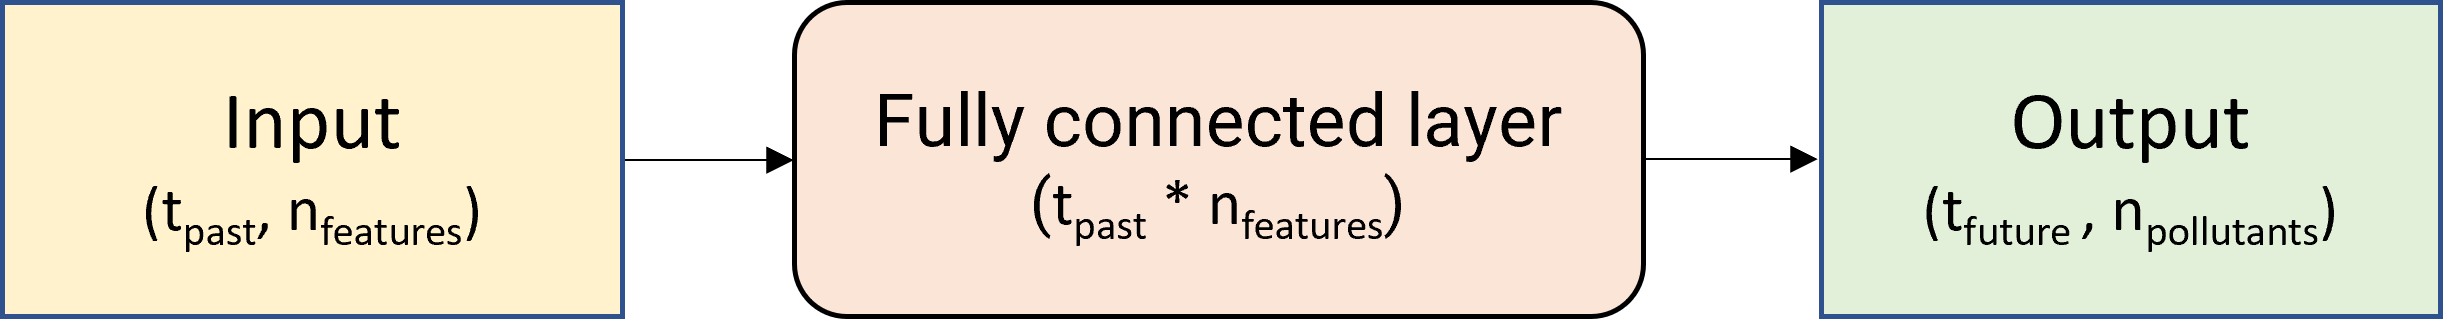
\includegraphics[width=0.7\linewidth]{images/model architectures/linearmodel.png}
    \caption{Proposed linear model architecture. The model takes an input matrix of size t\textsubscript{past} dimensions by features, and employs an MLP with no hidden layers to yield an output matrix sized t\textsubscript{future} dimensions by pollutants.}
    \label{fig:linearmodel}
\end{figure}

\subsection{LSTM model}

LSTMs (Long Short-term Memory) networks were introduced in 1997 by Sepp Hochreiter and Jürgen Schmidhuber \cite{hochreiter}. LSTM networks were created with the explicit purpose of addressing the challenge of long-term dependencies encountered by recurrent neural networks (RNNs), primarily stemming from the \textbf{vanishing gradient problem}\footnote{
In the process of training a recurrent neural network (RNN), the backpropagation algorithm moves in a backward direction from the output layer to the input layer. However, a common issue arises during this progression known as the \textbf{vanishing gradients problem}. As the algorithm descends, the gradients tend to diminish and become shallower, approaching zero. This phenomenon has a significant impact on the weights of the initial or lower layers, rendering them nearly unchanged. Consequently, the gradient descent optimization struggles to converge to the optimum solution. }. Distinguishing themselves from conventional feedforward neural networks, LSTMs incorporate feedback connections. This unique attribute empowers LSTMs to analyze entire sequences of data, such as time series, in a manner that goes beyond treating each point in the sequence in isolation. Instead, LSTMs retain valuable information from preceding data points in the sequence, facilitating the handling of new data points. Consequently, LSTMs excel in processing sequential data, making them particularly effective for tasks involving text, speech, and general time-series analysis.
The proposed model comprises two LSTM layers, each consisting of 50 LSTM units, arranged in a stacked configuration, wherein the output of the first layer serves as the input to the second. This architectural arrangement confers advantages by facilitating the acquisition of hierarchical representations of successive observations and enabling the detection of latent patterns within the data. Dropout regularization is applied following both LSTM layers, employing a rate of 0.4. Dropout is a regularization technique that stochastically sets input units to zero with a specified frequency (0.4 in this instance) during each training iteration, mitigating the risk of overfitting.
The output of the second LSTM layer yields, for each sample within the batch, a feature vector of dimensions 50. Subsequently, this feature vector is supplied to a dense linear layer for predictive modeling.

\begin{figure}
    \centering
    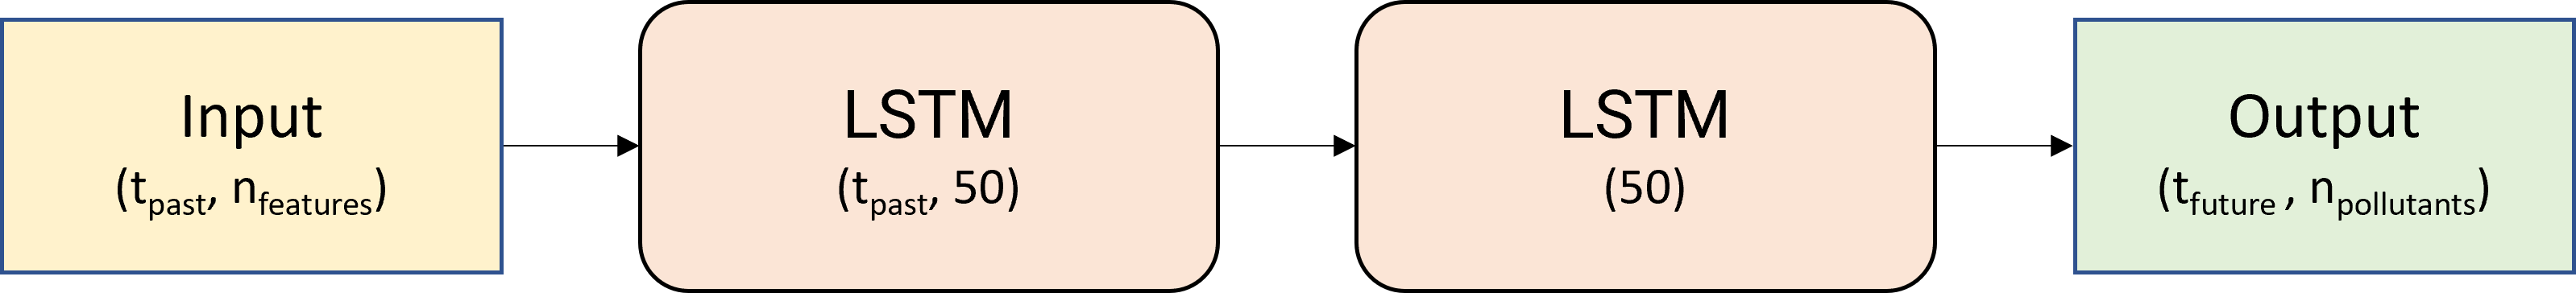
\includegraphics[width=0.7\linewidth]{images/model architectures/lstmmodel.png}
    \caption{Proposed LSTM model architecture. It involves processing an input matrix of size $t_{\text{past}}$ by features through two LSTM layers. The first LSTM layer generates an array of size 50 for each past time step, and the second LSTM layer produces a single feature vector of size 50. This vector is then passed to a dense linear layer, resulting in an output matrix of dimensions $t_{\text{future}}$ by pollutants.}
    \label{fig:lstmmodel}
\end{figure}

\subsection{Bidirectional LSTM model}


Bi-LSTM, short for Bidirectional Long Short-Term Memory, represents a variant of recurrent neural networks (RNNs) designed to effectively handle sequential data by processing it in both forward and backward directions.
The bidirectional processing of Bi-LSTM stands in contrast to one-directional processing in traditional RNNs \cite{Schuster1997BidirectionalRN}. Comprising two LSTM layers, one for forward and one for backward processing, each layer maintains its distinct hidden states and memory cells.
The forward pass involves feeding the input sequence into the forward LSTM layer, updating hidden states and memory cells at each time step based on current input and past information. Simultaneously, the backward pass processes the input sequence in reverse order, updating hidden states and memory cells based on current input and future context. After both passes, the hidden states from both LSTM layers are combined at each time step, enhancing the model's ability to capture comprehensive dependencies.

The proposed model is similar to the previous one, with the only difference being in the number of LSTM units in each layer (32 in the first one, and 64 in the second one), and the impementation of bidirectional processing in the two LSTM layers.

\begin{figure}
    \centering
    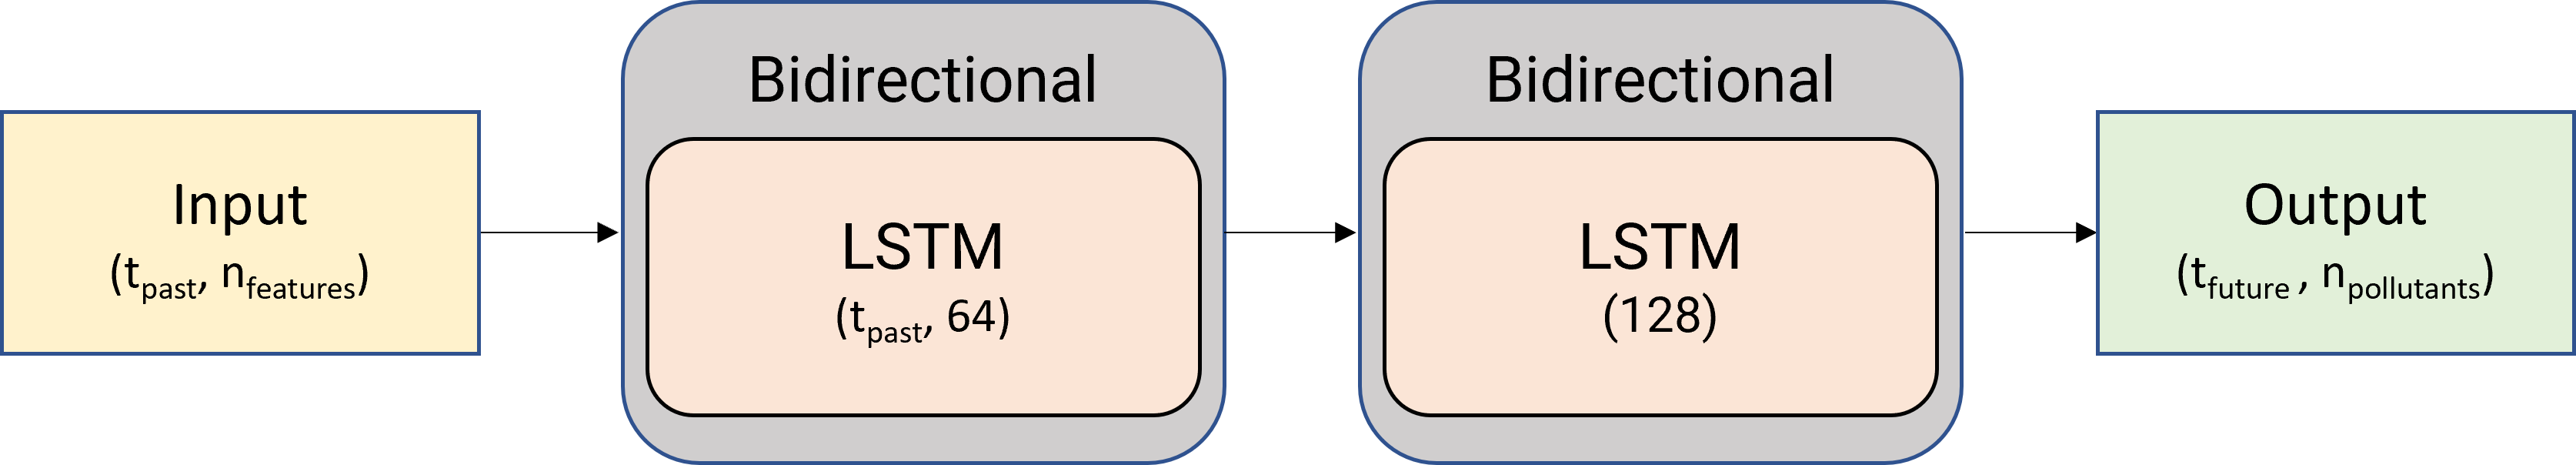
\includegraphics[width=0.7\linewidth]{images/model architectures/bilstmmodel.png}
    \caption{Proposed Bi-LSTM model architecture. It processes an input matrix of size $t_{\text{past}}$ by features, followed by two Bidirectional LSTM layers, first yielding a matrix of size $t_{\text{past}}$, 64, and the second one returning an array of size 128. Then the array is fed to a dense linear layer for predictions.
    }
    \label{fig:bilstmmodel}
\end{figure}

\subsection{Dense Encoder Decoder model}

The model is an autoencoder designed for sequential data. It consists of two blocks, encoder and decoder, each made only of dense layers.

\paragraph{Encoder Layers}
The encoder is responsible for transforming the input data into a more compact representation, often referred to as a latent space or encoding. It performs dimensionality reduction and extracts important features from the input. In the proposed model architecture, the encoder consists of several dense layers with non-linear activation functions (ReLU) and dropout layers. The final output of the encoder is a flattened representation that captures essential features of the input.
\begin{itemize}[noitemsep]
  \item Dense layer (128 units, ReLU activation)
  \item Dense layer (64 units, ReLU activation)
  \item Dense layer (32 units, ReLU activation)
\end{itemize}

\paragraph{Decoder Layers}
The decoder is tasked with reconstructing the original input data from the compressed representation generated by the encoder. It takes the encoded representation and transforms it back into the original format. In the model, the decoder comprises additional dense layers with non-linear activations and dropout layers. The final layer in the decoder produces the output, which is reshaped to match the dimensions of the original input.
\begin{itemize}[noitemsep]
  \item Dense layer (64 units, ReLU activation)
  \item Dense layer (128 units, ReLU activation)
  \item Dense layer (\( t_{\text{future}} \times n_{\text{pollutants}} \), linear activation)
\end{itemize}

\begin{figure}
    \centering
    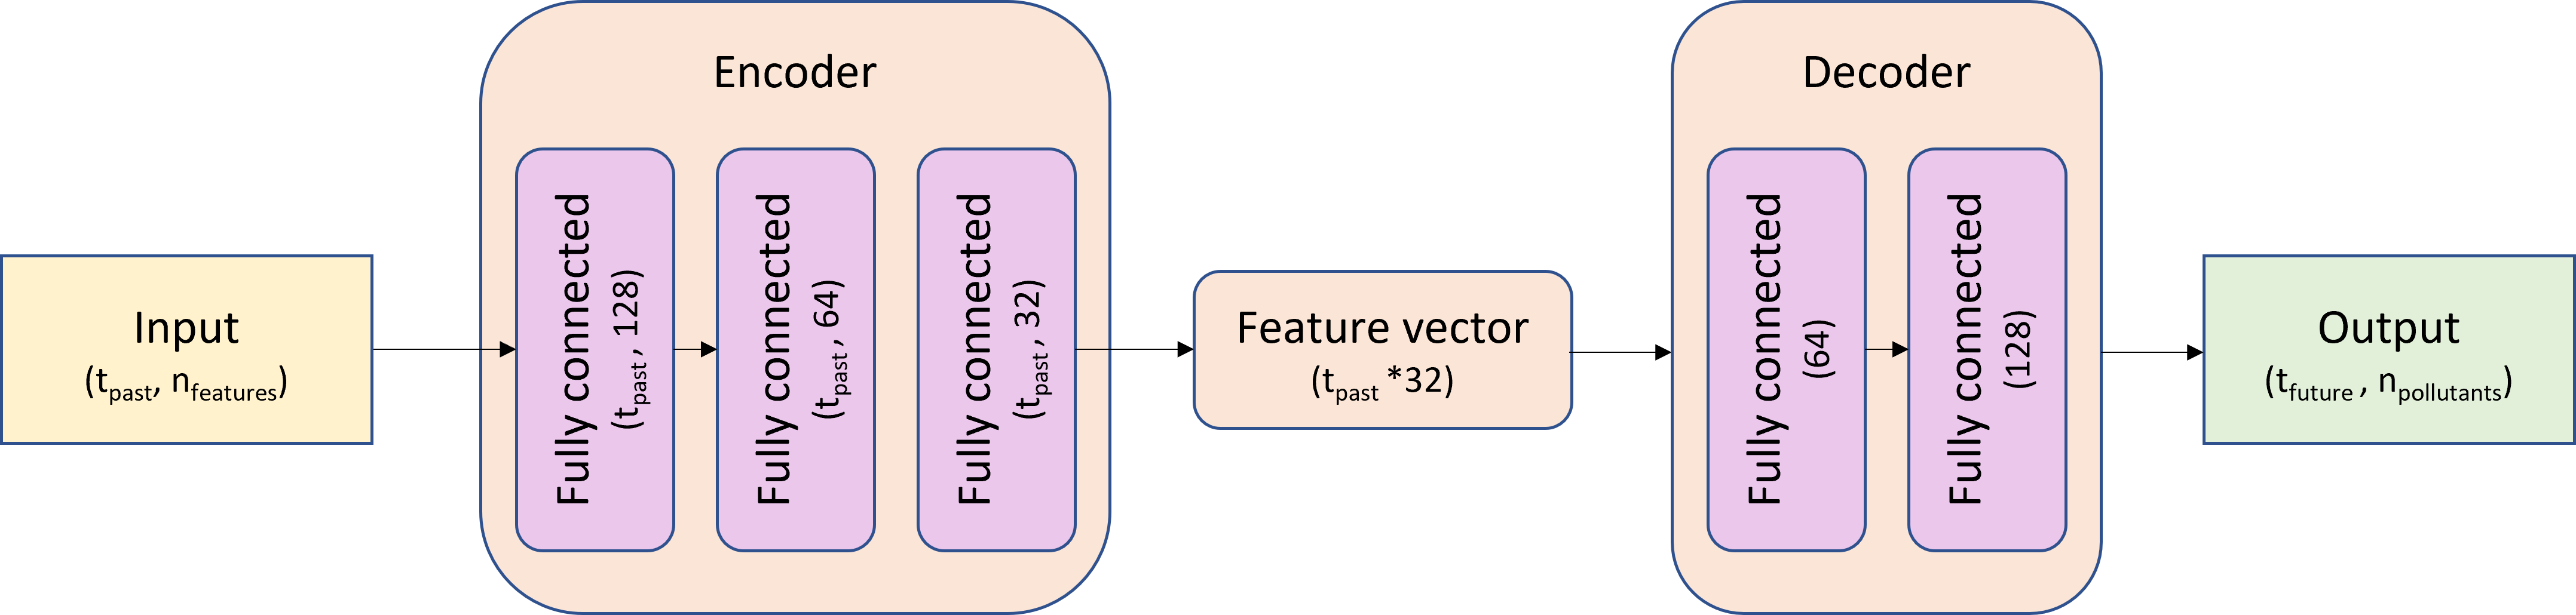
\includegraphics[width=1\linewidth]{images/model architectures/denseencdecmodel.png}
    \caption{Proposed Dense Encoder Decoder architecture}
    \label{fig:denseencdecmodel}
\end{figure}

The encoder effectively reduces the dimensionality of the input data, leading to more efficient storage and computation. Additionally, the model is adept at autonomously learning pertinent features from the input data without the need for explicit feature engineering. Dropout layers have been thoughtfully incorporated, serving as a means of regularization to prevent overfitting and augment the model's generalization capabilities.
One notable drawback lies in the fixed architecture of the model, being relatively simplistic and probably unable to adapt dynamically based on the complexity of the data. Another consideration is the potential loss of information during the compression process within the encoding layer. This is particularly relevant if the encoding dimension is too modest, possibly impacting the model's accuracy in faithfully reconstructing the input.

\subsection{CONV-LSTM model}

The proposed model architecture is a combination of Convolutional Neural Network (CNN) and Long Short-Term Memory (LSTM) layers. 
In the initial phase, the model processes input sequences of shape (t\textsubscript{past}, n\textsubscript{features}), where each sequence encapsulates t\textsubscript{past} time steps with n\textsubscript{features} features. The temporal dimension is then divided into seven segments, each representing a day, enabling isolated processing for daily patterns.
For each day, 1D convolutional layers with increasing filter sizes (64, 128, 256). Max pooling and batch normalization follow. Outputs from each day are concatenated along the temporal axis to capture dependencies.
The whole output is then passed through two consecutive LSTM layers, the first with 32 units and dropout (0.4), and the second with 64 units and another dropout layer. The final layer is a dense layer shaped for forecasting.

The combination of CNN and LSTM allows the model to capture both local patterns through convolutional operations and long-term dependencies through LSTM layers. By splitting the input sequence into daily segments, the model may better capture patterns specific to each day, potentially improving performance. Moreover, the use of causal padding in convolutional layers ensures that each output only depends on previous time steps, avoiding information leakage from the future.

However, due to it's complexity, this model could present some drawbacks such as the longer training times and the requirement of a larger amount of data for effective training, together with the risk of overfitting.


\begin{figure}
    \centering
    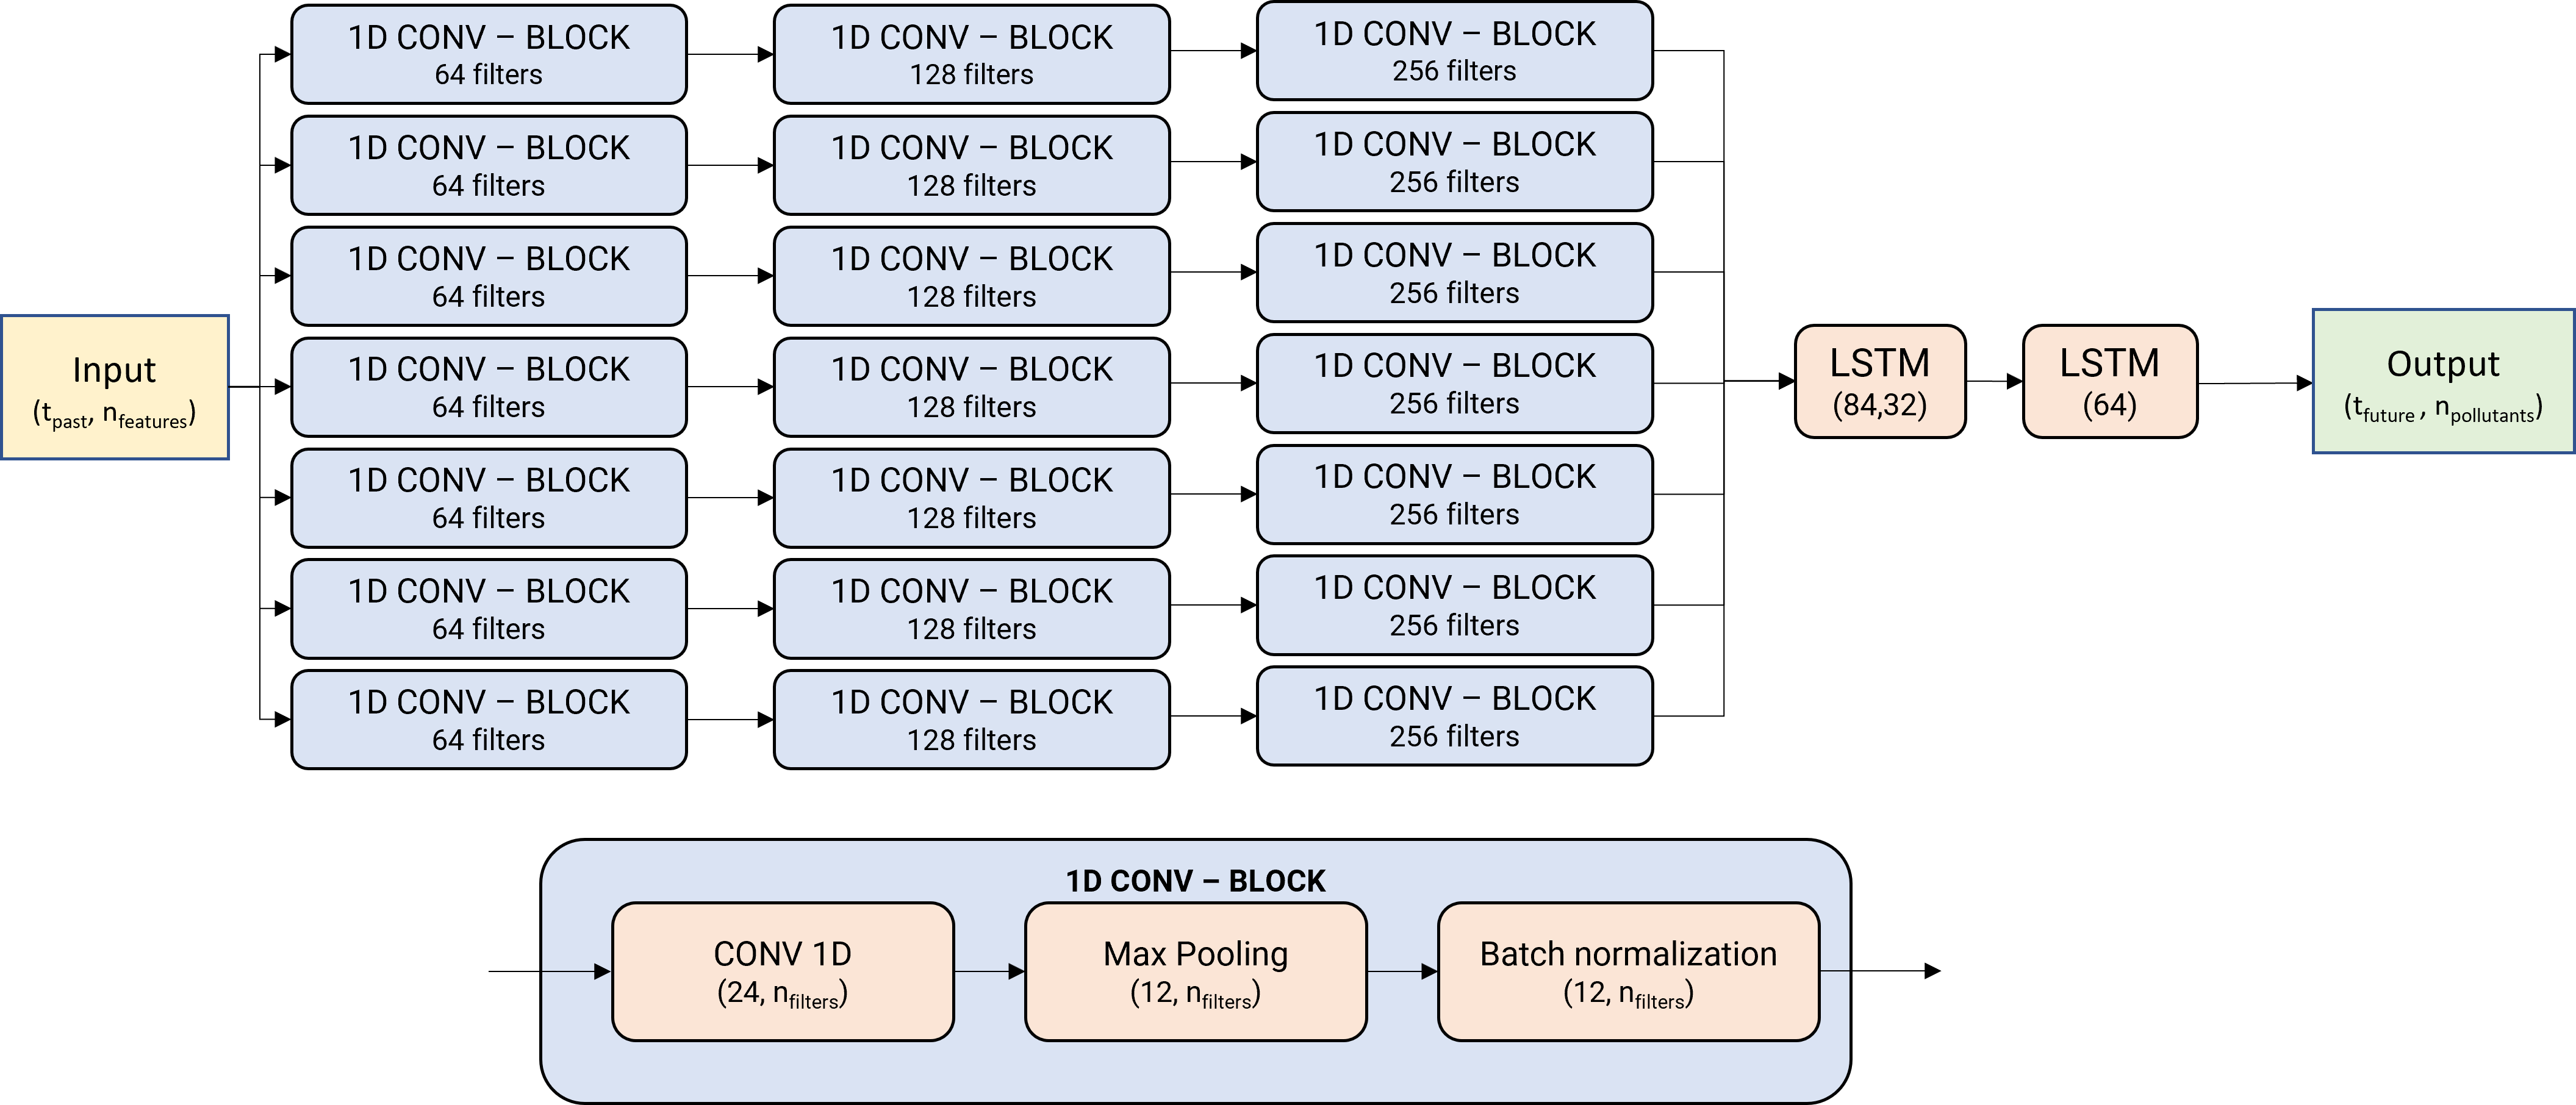
\includegraphics[width=1\linewidth]{images/model architectures/convlstm_model.png}
    \caption{Proposed CONV-LSTM architecture.}
    \label{fig:convlstm_model}
\end{figure}

\subsection{TSMixer model}

TSMixer, an abbreviation for Time-Series Mixer, presents an innovative architecture for time-series forecasting, employing a stacked arrangement of multi-layer perceptrons (MLPs). Documented in the paper entitled ``TSMixer: An All-MLP Architecture for Time Series Forecasting'' \cite{chen2023tsmixer}, this model diverges from prevailing and conventional methodologies in time-series forecasting. In contrast to contemporary approaches relying on high-capacity architectures like recurrent- or attention-based sequential deep learning models, TSMixer adopts a distinctive strategy by incorporating a sequence of multi-layer perceptrons in its design. The primary focus lies in amalgamating time and feature dimensions to enhance predictive accuracy. This discussion dissects the two principal components of TSMixer.

\paragraph{Mixer Layer}

The Mixer Layer serves as the locus for time mixing and feature mixing, encapsulating the essence of TSMixer's nomenclature.

\begin{figure}
    \centering
    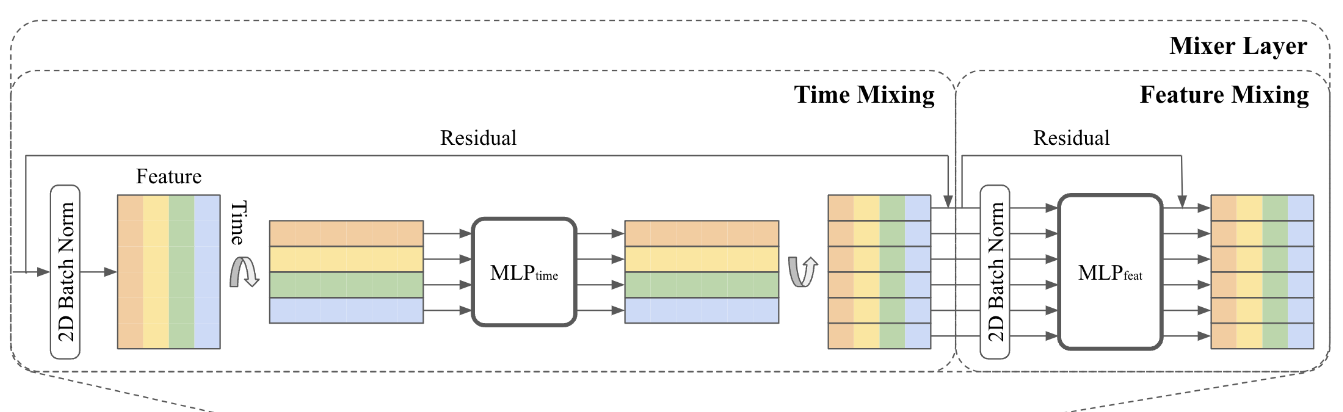
\includegraphics[width=1\linewidth]{images/model architectures/Mixing layer.png}
    \caption{Illustration of the mixing layer. \cite{chen2023tsmixer}}
    \label{fig:tsmixer-mixing-layer}
\end{figure}

The diagram above illustrates the mechanics of time mixing, wherein the MLP encompasses a fully connected layer, followed by the ReLU activation function, and a dropout layer. The input matrix, with rows representing time and columns representing features, undergoes transposition to facilitate the application of the MLP in the time domain, shared across all features. This unit is responsible for learning temporal patterns. Subsequent to exiting the time mixing unit, the matrix undergoes transposition once again before being directed to the feature mixing unit. The feature mixing unit comprises two MLPs and, being applied in the feature domain, is shared across all time steps. Noteworthy is the absence of the need for transposition, as the features are inherently aligned along the horizontal axis. Notably, both mixers incorporate normalization layers and residual connections. The latter aids the model in acquiring more profound representations of the data while maintaining computational efficiency, and normalization proves to be a conventional technique enhancing the training of deep learning models. Upon completion of the mixing process, the output proceeds to the temporal projection stage.

\paragraph{Temporal Projection}

\begin{figure}
    \centering
    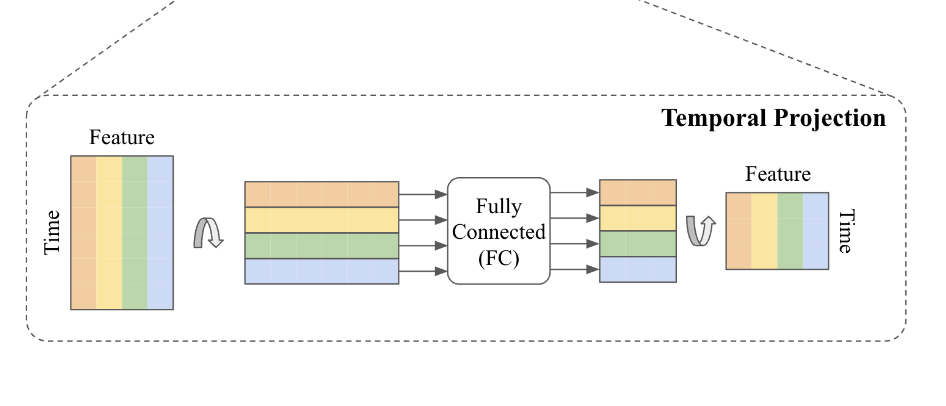
\includegraphics[width=1\linewidth]{images/model architectures/temporalprojection.png}
    \caption{Examination of the Temporal Projection. \cite{chen2023tsmixer}}
    \label{fig:enter-label}
\end{figure}

The Temporal Projection stage involves the retransposition of the matrix, followed by its passage through a fully connected layer to generate predictions. The ultimate step entails retransposing the matrix to arrange the features along the horizontal axis and the time steps along the vertical axis.

\begin{figure}
    \centering
    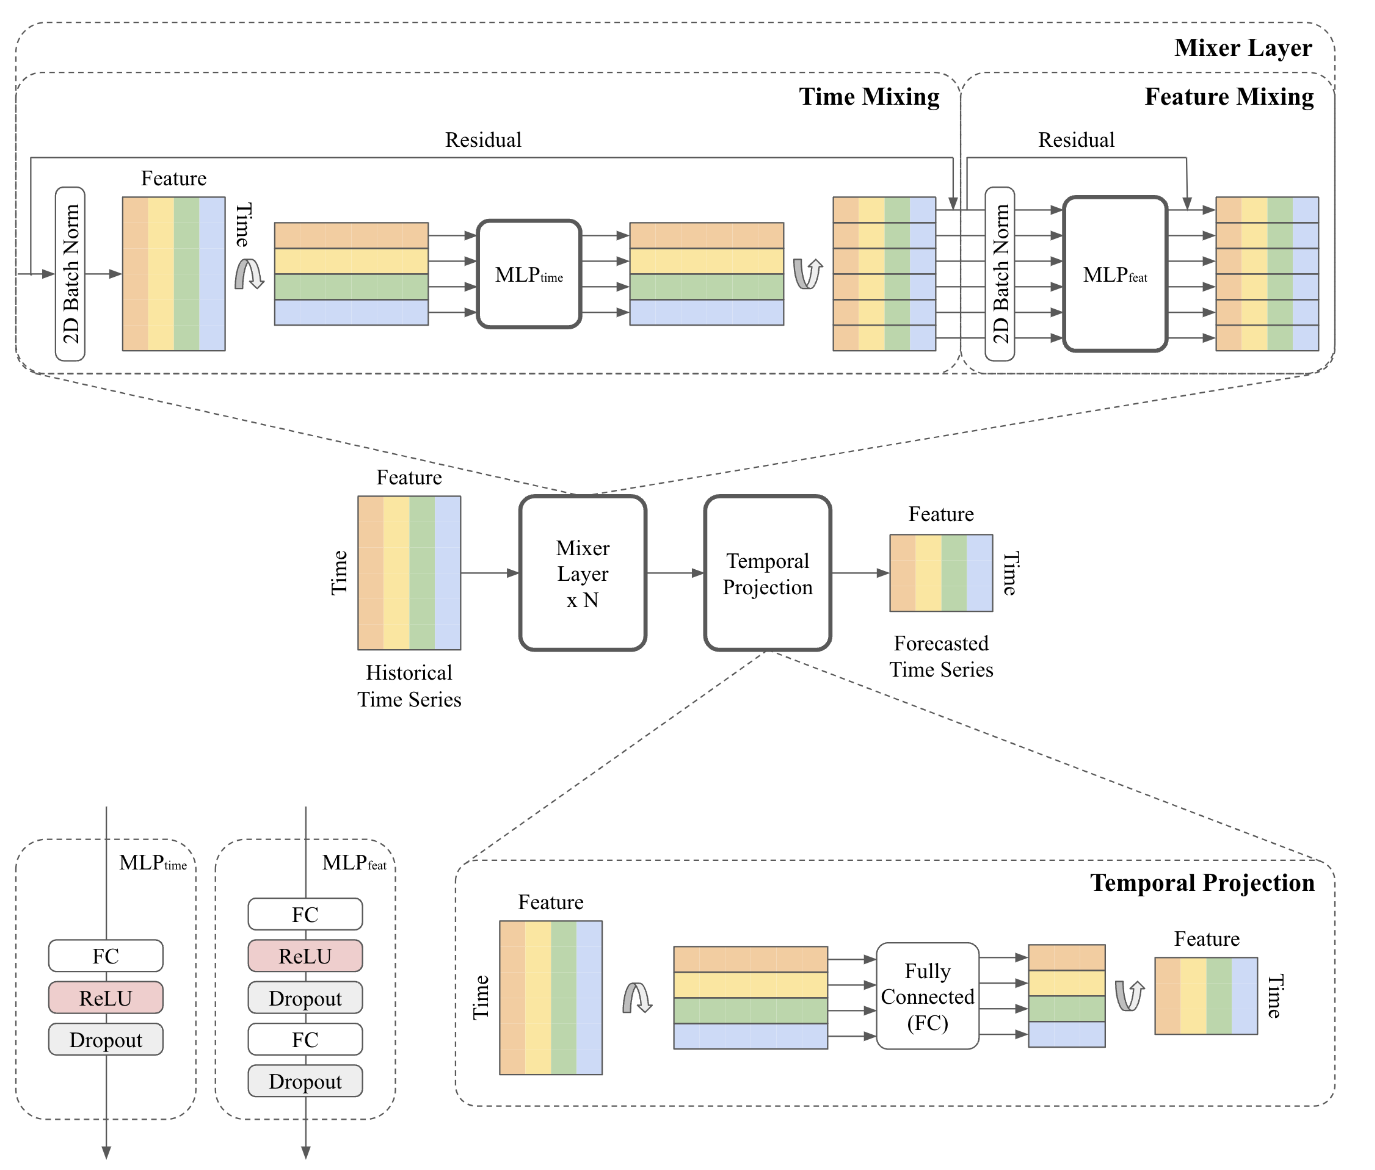
\includegraphics[width=1\linewidth]{images/model architectures/tsmixermodel.png}
    \caption{Comprehensive TSMixer architecture \cite{chen2023tsmixer}}
    \label{fig:tsmixer-whole architecture}
\end{figure}

The Tensorflow framework was used to implement the model. The proposed model concatenates 8 mixer layers before the temporal projection. This configuration results in heightened complexity, facilitating the capture of intricate patterns within the data. Notably, this heightened complexity does not come with an excessive increase in the number of parameters. Indeed, the model proves to be highly efficient, particularly when compared to the MLP architecture of the linear model.

\subsection{Wavelet model}

The developed wavelet model is a variant of the model proposed in \cite{WaveletNLSTM}. These two model takes advantage of Wavelet transform to decompose the signal into multiple wavelets, processing the components separatedly to capture more hidden patterns between the data.

\textbf{Wavelet transform} is a mathematical tool used for signal processing and analysis. It decomposes a signal into its constituent components called wavelets, which are small, well-localized functions with both time and frequency characteristics. Unlike traditional Fourier transform, which represents a signal as a sum of sinusoids of different frequencies, wavelet transform captures both time and frequency information simultaneously.
The wavelet transform involves passing the signal through a series of filters to extract different frequency components at various scales. The result of this process is a set of coefficients that represent the signal's behavior at different levels of detail and resolution.

In the proposed model, a Daubechies wavelet with one vanishing moment is employed, utilizing three levels of decomposition. The output of the decomposition consists of four arrays of different sizes, which represent the coefficients. These coefficients characterize distinct frequency components and details of the input signal across various scales. The approximation coefficients (cA1) encapsulate the low-frequency components, whereas the detail coefficients (cD1, cD2, cD3) encapsulate the high-frequency details at progressively higher levels of resolution. 


\begin{figure}
    \centering
    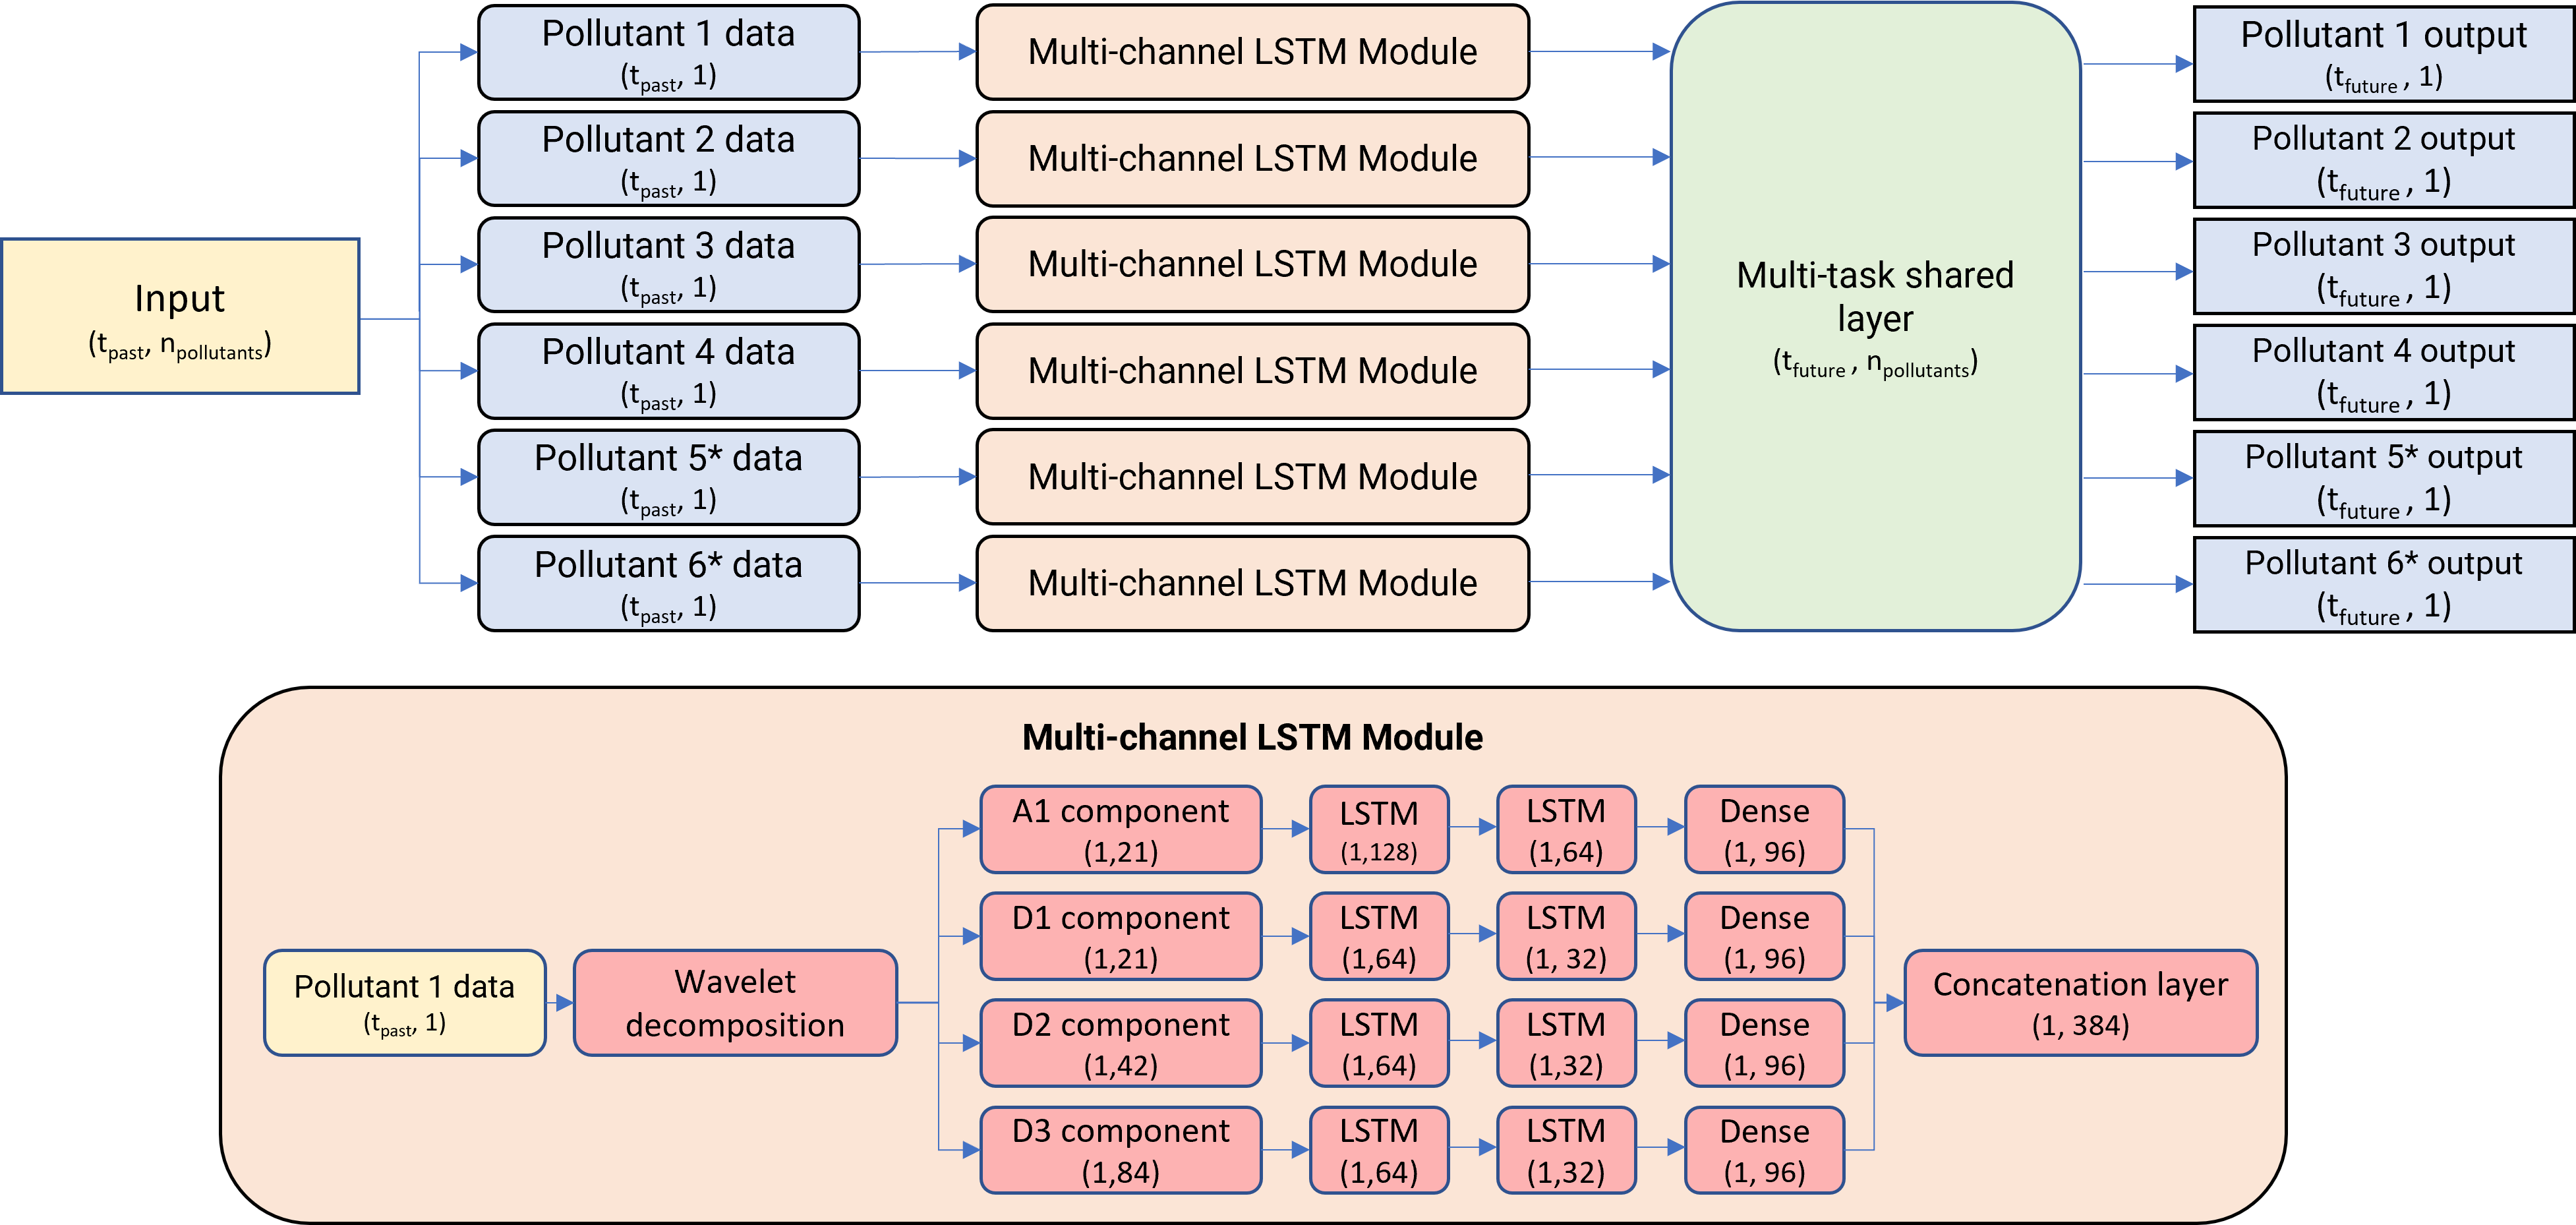
\includegraphics[width=1\linewidth]{images/model architectures/waveletmodel.png}
    \caption{Proposed Wavelet Model architecture}
    \label{fig:waveletmodel}
\end{figure}

The computational focal point is the Multi-channel LSTM module illustrated in Figure \ref{fig:waveletmodel}. Each component undergoes input to two consecutive LSTM layers, followed by processing through a dense layer for the normalization of individual component outcomes. Subsequently, the outputs from each module are consolidated in a shared layer, serving as the basis for the final predictions pertaining to pollutant levels.

\section{Model Evaluation and Training Details}

\subsection{Metrics}

In this section we will shortly present the two metrics utilized to evaluate the performances of the models

\paragraph{Mean Absolute Error (MAE)}
MAE, or Mean Absolute Error, is a metric used to evaluate the accuracy of a forecasting model, particularly in the context of time series forecasting. It measures the average absolute difference between the actual and predicted values, providing a straightforward assessment of the magnitude of errors without considering their direction. In the context of time series forecasting, MAE is useful as it treats underpredictions and overpredictions equally. The formula for calculating MAE is given by:

\[
MAE = \frac{1}{n} \sum_{i=1}^{n} |y_i - \hat{y}_i|
\]

where:
\begin{itemize}[noitemsep, leftmargin=*]
\item[] $n \text{ is the number of observations in the time series,}$
\item[] $y_i \text{ is the actual value at time } i$, 
\item[] $\hat{y}_i \text{ is the predicted value at time } i$.
\end{itemize}

A lower MAE indicates better accuracy, suggesting that the model's predictions are closer to the actual values.

\paragraph{Symmetric Mean Absolute Percentage Error}
When it comes to measuring accuracy relative to the actual values, the most
popular metric is MAPE (the mean absolute percentage error). Whilst being very intuitive MAPE degenerates into positive infinity as soon as any of the actual values is zero. Even relatively small actual values can easily explode MAPE towards infinity. So, effectively, MAPE is meaningful only if all observations have relatively large actual values. 

In this work context, sMAPE is preferred because it addresses the issue of scale, making it suitable for comparing accuracy across different time series with varying levels of magnitude, like ours. Moreover, sMAPE overcomes the MAPE limit of giving different weights in case of overestimation and underestimation. The formula for calculating sMAPE is calculated as follows:

\begin{equation}
sMAPE = \frac{100\%}{n} \sum_{t=1}^{n} \frac{|y_t - \hat{y}_t|}{( |y_t| + |\hat{y}_t| ) / 2}
\end{equation}

where:
\begin{itemize}[noitemsep,  leftmargin=*]
  \item[] \( n \) is the number of observations in the time series.
  \item[] \( y_t \) is the actual value at time \( t \).
  \item[] \( \hat{y}_t \) is the predicted value at time \( t \).
\end{itemize}

The formula calculates the absolute percentage error for each observation in the time series, averages these errors, and then expresses the result as a percentage. The division by \( (|y_t| + |\hat{y}_t|) / 2 \) ensures symmetry in the calculation, emphasizing both overestimation and underestimation errors equally. The sMAPE is expressed as a percentage, but it should not be interpreted as the percentage of the error due to its formulation. A perfect forecast is represented by 0\%, while higher percentages indicate a larger deviation between the actual and predicted values. The sMAPE can reach a maximum value of 200\%, and any value between 100\% and 200\% should be interpreted as an extremely high error.

\subsection{Training configuration}

When defining the training phase, it is important to consider several aspects that can affect the model's performance.
The first aspect to consider is the definition of a \textbf{loss function}. This function is used to update the weights of the neural network during the training phase, with the goal of minimizing or maximizing its value. In this case, the loss function chosen is the \textbf{Mean Squared Error} (MSE). It is calculated by taking the average of the squared differences between the predicted and actual values (refer to Figure \ref{eq:mse}).

\begin{figure}
\[MSE = \frac{1}{n} \sum_{t=1}^{n} (y_t - \hat{y}_t)^2\]
\caption{Mean Squared error formula}
\label{eq:mse}
\end{figure}

where:
\begin{itemize}[noitemsep, leftmargin=*]
  \item[] \( n \) is the number of observations in the time series,
  \item[] \( y_t \) represents the actual value at time \( t \),
  \item[] \( \hat{y}_t \) represents the predicted value at time \( t \), and
  \item[] The summation is taken over all time points from \( t = 1 \) to \( t = n \).
\end{itemize}

The second aspect to consider is the \textbf{optimizer} of the neural network and it's starting learning rate. The optimization algorithm employed in the training of forecasting models is \textbf{Adam} \cite{kingma2017adam}, an abbreviation for Adaptive Moment Estimation. Adam represents an adaptive learning rate optimization algorithm that amalgamates the merits of two well-established optimizers, namely Adagrad and RMSprop. Widely recognized as one of the preeminent optimizers for the training of deep neural networks, Adam is characterized by its capacity to dynamically adjust learning rates for individual parameters. This adaptive characteristic facilitates expedited convergence and enhanced optimization outcomes in practical applications. Adam's adaptability makes it ideal for tasks with fluctuating gradient magnitudes, helping to alleviate challenges such as vanishing or exploding gradient problems commonly encountered in deep learning. The optimal \textbf{learning rate} for all networks during testing was \textbf{0.001}.

To improve efficiency and monitoring during training, various \textbf{callbacks} were implemented:

\begin{itemize}
    \item \textbf{Plot Learning}: Visualizing learning through plots helps understand the evolution of a model. Learning curves, one for training and validation loss, and another one for training and validation MAE, provide insights into performance and identify issues like overfitting or underfitting.

    \item \textbf{Reduce Learning Rate on Plateau}: Dynamic adjustment of the learning rate during training enhances model convergence. This technique involves monitoring a metric (validation loss), reducing the learning rate by a factor of 0.8 if there's no improvement for 3 consecutive epochs, allowing delicate parameter fine-tuning and potential escape from local minima.

    \item \textbf{Early Stopping}: A regularization technique, early stopping halts training when a model's performance on a validation set degrades. Instead of training for a fixed number of epochs, training stops when there's no further improvement in the validation loss for 5 epochs, preventing overfitting and conserving computational resources.
\end{itemize}